% Options for packages loaded elsewhere
\PassOptionsToPackage{unicode}{hyperref}
\PassOptionsToPackage{hyphens}{url}
%
\documentclass[
]{article}
\usepackage{amsmath,amssymb}
\usepackage{lmodern}
\usepackage{iftex}
\ifPDFTeX
  \usepackage[T1]{fontenc}
  \usepackage[utf8]{inputenc}
  \usepackage{textcomp} % provide euro and other symbols
\else % if luatex or xetex
  \usepackage{unicode-math}
  \defaultfontfeatures{Scale=MatchLowercase}
  \defaultfontfeatures[\rmfamily]{Ligatures=TeX,Scale=1}
\fi
% Use upquote if available, for straight quotes in verbatim environments
\IfFileExists{upquote.sty}{\usepackage{upquote}}{}
\IfFileExists{microtype.sty}{% use microtype if available
  \usepackage[]{microtype}
  \UseMicrotypeSet[protrusion]{basicmath} % disable protrusion for tt fonts
}{}
\makeatletter
\@ifundefined{KOMAClassName}{% if non-KOMA class
  \IfFileExists{parskip.sty}{%
    \usepackage{parskip}
  }{% else
    \setlength{\parindent}{0pt}
    \setlength{\parskip}{6pt plus 2pt minus 1pt}}
}{% if KOMA class
  \KOMAoptions{parskip=half}}
\makeatother
\usepackage{xcolor}
\usepackage[margin=1in]{geometry}
\usepackage{color}
\usepackage{fancyvrb}
\newcommand{\VerbBar}{|}
\newcommand{\VERB}{\Verb[commandchars=\\\{\}]}
\DefineVerbatimEnvironment{Highlighting}{Verbatim}{commandchars=\\\{\}}
% Add ',fontsize=\small' for more characters per line
\usepackage{framed}
\definecolor{shadecolor}{RGB}{248,248,248}
\newenvironment{Shaded}{\begin{snugshade}}{\end{snugshade}}
\newcommand{\AlertTok}[1]{\textcolor[rgb]{0.94,0.16,0.16}{#1}}
\newcommand{\AnnotationTok}[1]{\textcolor[rgb]{0.56,0.35,0.01}{\textbf{\textit{#1}}}}
\newcommand{\AttributeTok}[1]{\textcolor[rgb]{0.77,0.63,0.00}{#1}}
\newcommand{\BaseNTok}[1]{\textcolor[rgb]{0.00,0.00,0.81}{#1}}
\newcommand{\BuiltInTok}[1]{#1}
\newcommand{\CharTok}[1]{\textcolor[rgb]{0.31,0.60,0.02}{#1}}
\newcommand{\CommentTok}[1]{\textcolor[rgb]{0.56,0.35,0.01}{\textit{#1}}}
\newcommand{\CommentVarTok}[1]{\textcolor[rgb]{0.56,0.35,0.01}{\textbf{\textit{#1}}}}
\newcommand{\ConstantTok}[1]{\textcolor[rgb]{0.00,0.00,0.00}{#1}}
\newcommand{\ControlFlowTok}[1]{\textcolor[rgb]{0.13,0.29,0.53}{\textbf{#1}}}
\newcommand{\DataTypeTok}[1]{\textcolor[rgb]{0.13,0.29,0.53}{#1}}
\newcommand{\DecValTok}[1]{\textcolor[rgb]{0.00,0.00,0.81}{#1}}
\newcommand{\DocumentationTok}[1]{\textcolor[rgb]{0.56,0.35,0.01}{\textbf{\textit{#1}}}}
\newcommand{\ErrorTok}[1]{\textcolor[rgb]{0.64,0.00,0.00}{\textbf{#1}}}
\newcommand{\ExtensionTok}[1]{#1}
\newcommand{\FloatTok}[1]{\textcolor[rgb]{0.00,0.00,0.81}{#1}}
\newcommand{\FunctionTok}[1]{\textcolor[rgb]{0.00,0.00,0.00}{#1}}
\newcommand{\ImportTok}[1]{#1}
\newcommand{\InformationTok}[1]{\textcolor[rgb]{0.56,0.35,0.01}{\textbf{\textit{#1}}}}
\newcommand{\KeywordTok}[1]{\textcolor[rgb]{0.13,0.29,0.53}{\textbf{#1}}}
\newcommand{\NormalTok}[1]{#1}
\newcommand{\OperatorTok}[1]{\textcolor[rgb]{0.81,0.36,0.00}{\textbf{#1}}}
\newcommand{\OtherTok}[1]{\textcolor[rgb]{0.56,0.35,0.01}{#1}}
\newcommand{\PreprocessorTok}[1]{\textcolor[rgb]{0.56,0.35,0.01}{\textit{#1}}}
\newcommand{\RegionMarkerTok}[1]{#1}
\newcommand{\SpecialCharTok}[1]{\textcolor[rgb]{0.00,0.00,0.00}{#1}}
\newcommand{\SpecialStringTok}[1]{\textcolor[rgb]{0.31,0.60,0.02}{#1}}
\newcommand{\StringTok}[1]{\textcolor[rgb]{0.31,0.60,0.02}{#1}}
\newcommand{\VariableTok}[1]{\textcolor[rgb]{0.00,0.00,0.00}{#1}}
\newcommand{\VerbatimStringTok}[1]{\textcolor[rgb]{0.31,0.60,0.02}{#1}}
\newcommand{\WarningTok}[1]{\textcolor[rgb]{0.56,0.35,0.01}{\textbf{\textit{#1}}}}
\usepackage{graphicx}
\makeatletter
\def\maxwidth{\ifdim\Gin@nat@width>\linewidth\linewidth\else\Gin@nat@width\fi}
\def\maxheight{\ifdim\Gin@nat@height>\textheight\textheight\else\Gin@nat@height\fi}
\makeatother
% Scale images if necessary, so that they will not overflow the page
% margins by default, and it is still possible to overwrite the defaults
% using explicit options in \includegraphics[width, height, ...]{}
\setkeys{Gin}{width=\maxwidth,height=\maxheight,keepaspectratio}
% Set default figure placement to htbp
\makeatletter
\def\fps@figure{htbp}
\makeatother
\setlength{\emergencystretch}{3em} % prevent overfull lines
\providecommand{\tightlist}{%
  \setlength{\itemsep}{0pt}\setlength{\parskip}{0pt}}
\setcounter{secnumdepth}{-\maxdimen} % remove section numbering
\ifLuaTeX
  \usepackage{selnolig}  % disable illegal ligatures
\fi
\IfFileExists{bookmark.sty}{\usepackage{bookmark}}{\usepackage{hyperref}}
\IfFileExists{xurl.sty}{\usepackage{xurl}}{} % add URL line breaks if available
\urlstyle{same} % disable monospaced font for URLs
\hypersetup{
  pdftitle={Final\_proj\_8106},
  hidelinks,
  pdfcreator={LaTeX via pandoc}}

\title{Final\_proj\_8106}
\author{}
\date{\vspace{-2.5em}2023-05-06}

\begin{document}
\maketitle

\newpage
\newpage

\begin{Shaded}
\begin{Highlighting}[]
\FunctionTok{library}\NormalTok{(caret)}
\FunctionTok{library}\NormalTok{(mlbench)}
\FunctionTok{library}\NormalTok{(pdp)}
\FunctionTok{library}\NormalTok{(vip)}
\FunctionTok{library}\NormalTok{(AppliedPredictiveModeling)}
\FunctionTok{library}\NormalTok{(tidyverse)}
\FunctionTok{library}\NormalTok{(klaR)}
\FunctionTok{library}\NormalTok{(MASS)}
\FunctionTok{library}\NormalTok{(corrplot)}
\FunctionTok{library}\NormalTok{(plotmo)}
\FunctionTok{library}\NormalTok{(ggplot2)}
\FunctionTok{library}\NormalTok{(pls)}
\FunctionTok{library}\NormalTok{(ggpubr)}
\FunctionTok{library}\NormalTok{(factoextra)}
\FunctionTok{library}\NormalTok{(gridExtra)}
\FunctionTok{library}\NormalTok{(corrplot)}
\FunctionTok{library}\NormalTok{(RColorBrewer) }
\FunctionTok{library}\NormalTok{(gplots)}
\FunctionTok{library}\NormalTok{(jpeg)}
\FunctionTok{library}\NormalTok{(rpart.plot)}
\FunctionTok{library}\NormalTok{(randomForest)}
\FunctionTok{library}\NormalTok{(ranger)}
\FunctionTok{library}\NormalTok{(gbm)}
\FunctionTok{library}\NormalTok{(pROC)}
\end{Highlighting}
\end{Shaded}

\begin{Shaded}
\begin{Highlighting}[]
\CommentTok{\# import and subset data}
\FunctionTok{load}\NormalTok{(}\StringTok{"./recovery.RData"}\NormalTok{)}
\FunctionTok{set.seed}\NormalTok{(}\DecValTok{5095}\NormalTok{)}
\NormalTok{dat}\FloatTok{.1} \OtherTok{=}\NormalTok{ dat[}\FunctionTok{sample}\NormalTok{(}\DecValTok{1}\SpecialCharTok{:}\DecValTok{10000}\NormalTok{, }\DecValTok{2000}\NormalTok{),]}

\FunctionTok{set.seed}\NormalTok{(}\DecValTok{5296}\NormalTok{)}
\NormalTok{dat}\FloatTok{.2} \OtherTok{=}\NormalTok{ dat[}\FunctionTok{sample}\NormalTok{(}\DecValTok{1}\SpecialCharTok{:}\DecValTok{10000}\NormalTok{, }\DecValTok{2000}\NormalTok{),]}

\NormalTok{dat.all }\OtherTok{=} \FunctionTok{rbind}\NormalTok{(dat}\FloatTok{.1}\NormalTok{, dat}\FloatTok{.2}\NormalTok{)}\SpecialCharTok{\%\textgreater{}\%}
  \FunctionTok{unique.array}\NormalTok{()}

\CommentTok{\# transform variables as needed}
\NormalTok{dat1 }\OtherTok{=}\NormalTok{ dat.all[}\DecValTok{2}\SpecialCharTok{:}\DecValTok{16}\NormalTok{] }\SpecialCharTok{\%\textgreater{}\%} 
  \FunctionTok{mutate}\NormalTok{(}\AttributeTok{gender =} \FunctionTok{as.factor}\NormalTok{(gender), }
         \AttributeTok{race =} \FunctionTok{as.factor}\NormalTok{(race),}
         \AttributeTok{smoking =} \FunctionTok{as.factor}\NormalTok{(smoking),}
         \AttributeTok{hypertension =} \FunctionTok{as.factor}\NormalTok{(hypertension),}
         \AttributeTok{diabetes =} \FunctionTok{as.factor}\NormalTok{(diabetes),}
         \AttributeTok{vaccine =} \FunctionTok{as.factor}\NormalTok{(vaccine),}
         \AttributeTok{severity =} \FunctionTok{as.factor}\NormalTok{(severity),}
         \AttributeTok{study =} \FunctionTok{as.factor}\NormalTok{(study))   }

\CommentTok{\# transform into matrix}
\NormalTok{dat2 }\OtherTok{=} \FunctionTok{model.matrix}\NormalTok{(recovery\_time }\SpecialCharTok{\textasciitilde{}}\NormalTok{ ., dat1)[ ,}\SpecialCharTok{{-}}\DecValTok{1}\NormalTok{]}

\CommentTok{\# split data into training set and test set}
\FunctionTok{set.seed}\NormalTok{(}\DecValTok{1}\NormalTok{)}
\NormalTok{trainRows }\OtherTok{=} \FunctionTok{createDataPartition}\NormalTok{(}\AttributeTok{y =}\NormalTok{ dat1}\SpecialCharTok{$}\NormalTok{recovery\_time, }\AttributeTok{p =} \FloatTok{0.8}\NormalTok{, }\AttributeTok{list =} \ConstantTok{FALSE}\NormalTok{)}
\end{Highlighting}
\end{Shaded}

\begin{Shaded}
\begin{Highlighting}[]
\CommentTok{\# extract training data}
\NormalTok{x.train }\OtherTok{=}\NormalTok{ dat2[trainRows,]}
\NormalTok{y.train }\OtherTok{=}\NormalTok{ dat1}\SpecialCharTok{$}\NormalTok{recovery\_time[trainRows]}

\CommentTok{\# correlation plot}
\NormalTok{x\_cor }\OtherTok{=}\NormalTok{ dat2[trainRows, }\FunctionTok{c}\NormalTok{(}\StringTok{"age"}\NormalTok{, }\StringTok{"height"}\NormalTok{, }\StringTok{"weight"}\NormalTok{, }\StringTok{"bmi"}\NormalTok{, }\StringTok{"SBP"}\NormalTok{, }\StringTok{"LDL"}\NormalTok{)]}
\FunctionTok{png}\NormalTok{(}\AttributeTok{height=}\DecValTok{1800}\NormalTok{, }\AttributeTok{width=}\DecValTok{1800}\NormalTok{, }\AttributeTok{units =} \StringTok{"px"}\NormalTok{, }\AttributeTok{file=}\StringTok{"corrplot.png"}\NormalTok{, }\AttributeTok{res =} \DecValTok{200}\NormalTok{)}
\NormalTok{corrplot}\SpecialCharTok{::}\FunctionTok{corrplot}\NormalTok{(}\FunctionTok{cor}\NormalTok{(x\_cor), }\AttributeTok{method =} \StringTok{"circle"}\NormalTok{, }\AttributeTok{type =} \StringTok{"full"}\NormalTok{)}
\FunctionTok{dev.off}\NormalTok{()}
\end{Highlighting}
\end{Shaded}

\begin{verbatim}
## pdf 
##   2
\end{verbatim}

\begin{Shaded}
\begin{Highlighting}[]
\CommentTok{\#library("PerformanceAnalytics")}
\CommentTok{\#chart.Correlation(x, histogram=TRUE, pch=19)}

\NormalTok{x.test }\OtherTok{=}\NormalTok{ dat2[}\SpecialCharTok{{-}}\NormalTok{trainRows,]}
\NormalTok{y.test }\OtherTok{=}\NormalTok{ dat1}\SpecialCharTok{$}\NormalTok{recovery\_time[}\SpecialCharTok{{-}}\NormalTok{trainRows]}

\CommentTok{\# plot numeric variables}
\NormalTok{theme1 }\OtherTok{\textless{}{-}} \FunctionTok{trellis.par.get}\NormalTok{()}
\NormalTok{theme1}\SpecialCharTok{$}\NormalTok{plot.symbol}\SpecialCharTok{$}\NormalTok{col }\OtherTok{\textless{}{-}} \FunctionTok{rgb}\NormalTok{(.}\DecValTok{2}\NormalTok{, .}\DecValTok{4}\NormalTok{, .}\DecValTok{2}\NormalTok{, .}\DecValTok{5}\NormalTok{)}
\NormalTok{theme1}\SpecialCharTok{$}\NormalTok{plot.symbol}\SpecialCharTok{$}\NormalTok{pch }\OtherTok{\textless{}{-}} \DecValTok{16}
\NormalTok{theme1}\SpecialCharTok{$}\NormalTok{plot.line}\SpecialCharTok{$}\NormalTok{col }\OtherTok{\textless{}{-}} \FunctionTok{rgb}\NormalTok{(.}\DecValTok{8}\NormalTok{, .}\DecValTok{1}\NormalTok{, .}\DecValTok{1}\NormalTok{, }\DecValTok{1}\NormalTok{)}
\NormalTok{theme1}\SpecialCharTok{$}\NormalTok{plot.line}\SpecialCharTok{$}\NormalTok{lwd }\OtherTok{\textless{}{-}} \DecValTok{2}
\NormalTok{theme1}\SpecialCharTok{$}\NormalTok{strip.background}\SpecialCharTok{$}\NormalTok{col }\OtherTok{\textless{}{-}} \FunctionTok{rgb}\NormalTok{(.}\DecValTok{0}\NormalTok{, .}\DecValTok{2}\NormalTok{, .}\DecValTok{6}\NormalTok{, .}\DecValTok{2}\NormalTok{)}
\FunctionTok{trellis.par.set}\NormalTok{(theme1)}

\FunctionTok{png}\NormalTok{(}\AttributeTok{height=}\DecValTok{1800}\NormalTok{, }\AttributeTok{width=}\DecValTok{1800}\NormalTok{, }\AttributeTok{units =} \StringTok{"px"}\NormalTok{, }\AttributeTok{file=}\StringTok{"featureplot.png"}\NormalTok{, }\AttributeTok{res =} \DecValTok{200}\NormalTok{)}
\NormalTok{p1 }\OtherTok{=} \FunctionTok{featurePlot}\NormalTok{(x.train[,}\FunctionTok{c}\NormalTok{(}\DecValTok{1}\NormalTok{,}\DecValTok{8}\NormalTok{, }\DecValTok{9}\NormalTok{, }\DecValTok{10}\NormalTok{, }\DecValTok{13}\NormalTok{, }\DecValTok{14}\NormalTok{)], y.train, }\AttributeTok{plot =} \StringTok{"scatter"}\NormalTok{, }\AttributeTok{labels =} \FunctionTok{c}\NormalTok{(}\StringTok{""}\NormalTok{,}\StringTok{"Y"}\NormalTok{),}
            \AttributeTok{type =} \FunctionTok{c}\NormalTok{(}\StringTok{"p"}\NormalTok{), }\AttributeTok{layout =} \FunctionTok{c}\NormalTok{(}\DecValTok{3}\NormalTok{, }\DecValTok{2}\NormalTok{))}
\NormalTok{p1}
\FunctionTok{dev.off}\NormalTok{()}
\end{Highlighting}
\end{Shaded}

\begin{verbatim}
## pdf 
##   2
\end{verbatim}

\begin{Shaded}
\begin{Highlighting}[]
\CommentTok{\# plot categorical variables}
\NormalTok{p2 }\OtherTok{=} \FunctionTok{ggplot}\NormalTok{(dat1, }\FunctionTok{aes}\NormalTok{(}\AttributeTok{y =}\NormalTok{ recovery\_time, }\AttributeTok{x =}\NormalTok{ gender))}\SpecialCharTok{+}
  \FunctionTok{geom\_boxplot}\NormalTok{()}
\NormalTok{p3 }\OtherTok{=} \FunctionTok{ggplot}\NormalTok{(dat1, }\FunctionTok{aes}\NormalTok{(}\AttributeTok{y =}\NormalTok{ recovery\_time, }\AttributeTok{x =}\NormalTok{ race))}\SpecialCharTok{+}
  \FunctionTok{geom\_boxplot}\NormalTok{()}
\NormalTok{p4 }\OtherTok{=} \FunctionTok{ggplot}\NormalTok{(dat1, }\FunctionTok{aes}\NormalTok{(}\AttributeTok{y =}\NormalTok{ recovery\_time, }\AttributeTok{x =}\NormalTok{ smoking))}\SpecialCharTok{+}
  \FunctionTok{geom\_boxplot}\NormalTok{()}
\NormalTok{p5 }\OtherTok{=} \FunctionTok{ggplot}\NormalTok{(dat1, }\FunctionTok{aes}\NormalTok{(}\AttributeTok{y =}\NormalTok{ recovery\_time, }\AttributeTok{x =}\NormalTok{ hypertension))}\SpecialCharTok{+}
  \FunctionTok{geom\_boxplot}\NormalTok{()}
\NormalTok{p6 }\OtherTok{=} \FunctionTok{ggplot}\NormalTok{(dat1, }\FunctionTok{aes}\NormalTok{(}\AttributeTok{y =}\NormalTok{ recovery\_time, }\AttributeTok{x =}\NormalTok{ diabetes))}\SpecialCharTok{+}
  \FunctionTok{geom\_boxplot}\NormalTok{()}
\NormalTok{p7 }\OtherTok{=} \FunctionTok{ggplot}\NormalTok{(dat1, }\FunctionTok{aes}\NormalTok{(}\AttributeTok{y =}\NormalTok{ recovery\_time, }\AttributeTok{x =}\NormalTok{ vaccine))}\SpecialCharTok{+}
  \FunctionTok{geom\_boxplot}\NormalTok{()}
\NormalTok{p8 }\OtherTok{=} \FunctionTok{ggplot}\NormalTok{(dat1, }\FunctionTok{aes}\NormalTok{(}\AttributeTok{y =}\NormalTok{ recovery\_time, }\AttributeTok{x =}\NormalTok{ severity))}\SpecialCharTok{+}
  \FunctionTok{geom\_boxplot}\NormalTok{()}
\NormalTok{p9 }\OtherTok{=} \FunctionTok{ggplot}\NormalTok{(dat1, }\FunctionTok{aes}\NormalTok{(}\AttributeTok{y =}\NormalTok{ recovery\_time, }\AttributeTok{x =}\NormalTok{ study))}\SpecialCharTok{+}
  \FunctionTok{geom\_boxplot}\NormalTok{()}

\NormalTok{arrange }\OtherTok{=} \FunctionTok{ggarrange}\NormalTok{(p2, p3, p4, p5, p6, p7, p8, p9, }\AttributeTok{ncol =} \DecValTok{4}\NormalTok{, }\AttributeTok{nrow =} \DecValTok{2}\NormalTok{)}
\FunctionTok{ggsave}\NormalTok{(}\StringTok{"arrangedplot.png"}\NormalTok{, arrange)}
\end{Highlighting}
\end{Shaded}

\begin{verbatim}
## Saving 6.5 x 4.5 in image
\end{verbatim}

\begin{Shaded}
\begin{Highlighting}[]
\NormalTok{ctrl1 }\OtherTok{=} \FunctionTok{trainControl}\NormalTok{(}\AttributeTok{method =} \StringTok{"cv"}\NormalTok{)}
\end{Highlighting}
\end{Shaded}

\hypertarget{linear-regression}{%
\subsection{Linear regression}\label{linear-regression}}

\begin{Shaded}
\begin{Highlighting}[]
\FunctionTok{set.seed}\NormalTok{(}\DecValTok{1}\NormalTok{)}
\NormalTok{lm.fit }\OtherTok{\textless{}{-}} \FunctionTok{train}\NormalTok{(x.train, y.train,}
                \AttributeTok{method =} \StringTok{"lm"}\NormalTok{,}
                \AttributeTok{trControl =}\NormalTok{ ctrl1)}
\FunctionTok{summary}\NormalTok{(lm.fit)}
\end{Highlighting}
\end{Shaded}

\begin{verbatim}
## 
## Call:
## lm(formula = .outcome ~ ., data = dat)
## 
## Residuals:
##     Min      1Q  Median      3Q     Max 
## -91.266 -14.386  -1.309  10.491 249.295 
## 
## Coefficients:
##                 Estimate Std. Error t value Pr(>|t|)    
## (Intercept)   -2.765e+03  1.328e+02 -20.816  < 2e-16 ***
## age            5.418e-02  1.163e-01   0.466   0.6413    
## gender1       -4.167e+00  9.375e-01  -4.445 9.13e-06 ***
## race2          8.711e-01  2.085e+00   0.418   0.6761    
## race3         -2.596e+00  1.195e+00  -2.173   0.0299 *  
## race4         -2.298e+00  1.582e+00  -1.453   0.1464    
## smoking1       5.844e+00  1.056e+00   5.536 3.38e-08 ***
## smoking2       7.779e+00  1.579e+00   4.926 8.87e-07 ***
## height         1.613e+01  7.826e-01  20.605  < 2e-16 ***
## weight        -1.751e+01  8.287e-01 -21.125  < 2e-16 ***
## bmi            5.288e+01  2.364e+00  22.366  < 2e-16 ***
## hypertension1  3.605e+00  1.589e+00   2.268   0.0234 *  
## diabetes1     -8.238e-01  1.292e+00  -0.638   0.5238    
## SBP            1.935e-02  1.046e-01   0.185   0.8533    
## LDL           -5.858e-02  2.480e-02  -2.362   0.0183 *  
## vaccine1      -7.888e+00  9.610e-01  -8.208 3.37e-16 ***
## severity1      8.905e+00  1.522e+00   5.852 5.40e-09 ***
## studyB         5.322e+00  1.207e+00   4.411 1.07e-05 ***
## studyC        -1.153e+00  1.453e+00  -0.794   0.4274    
## ---
## Signif. codes:  0 '***' 0.001 '**' 0.01 '*' 0.05 '.' 0.1 ' ' 1
## 
## Residual standard error: 25.08 on 2863 degrees of freedom
## Multiple R-squared:  0.2776, Adjusted R-squared:  0.2731 
## F-statistic: 61.12 on 18 and 2863 DF,  p-value: < 2.2e-16
\end{verbatim}

\hypertarget{ridge}{%
\subsection{Ridge}\label{ridge}}

\begin{Shaded}
\begin{Highlighting}[]
\FunctionTok{set.seed}\NormalTok{(}\DecValTok{1}\NormalTok{)}
\NormalTok{ridge.fit }\OtherTok{\textless{}{-}} \FunctionTok{train}\NormalTok{(x.train, y.train,}
                   \AttributeTok{method =} \StringTok{"glmnet"}\NormalTok{,}
                   \AttributeTok{tuneGrid =} \FunctionTok{expand.grid}\NormalTok{(}\AttributeTok{alpha =} \DecValTok{0}\NormalTok{, }
                                          \AttributeTok{lambda =} \FunctionTok{exp}\NormalTok{(}\FunctionTok{seq}\NormalTok{(}\DecValTok{10}\NormalTok{, }\SpecialCharTok{{-}}\DecValTok{5}\NormalTok{, }\AttributeTok{length=}\DecValTok{200}\NormalTok{))),}
                   \AttributeTok{preProc =} \FunctionTok{c}\NormalTok{(}\StringTok{"center"}\NormalTok{, }\StringTok{"scale"}\NormalTok{),}
                   \AttributeTok{trControl =}\NormalTok{ ctrl1)}
\end{Highlighting}
\end{Shaded}

\begin{verbatim}
## Warning in nominalTrainWorkflow(x = x, y = y, wts = weights, info = trainInfo,
## : There were missing values in resampled performance measures.
\end{verbatim}

\begin{Shaded}
\begin{Highlighting}[]
\FunctionTok{png}\NormalTok{(}\AttributeTok{file=}\StringTok{"ridge.tiff"}\NormalTok{, }\AttributeTok{height=}\DecValTok{1800}\NormalTok{, }\AttributeTok{width=}\DecValTok{1800}\NormalTok{, }\AttributeTok{units =} \StringTok{"px"}\NormalTok{, }\AttributeTok{res=}\DecValTok{200}\NormalTok{)}
\FunctionTok{plot}\NormalTok{(ridge.fit, }\AttributeTok{xTrans =}\NormalTok{ log)}
\FunctionTok{dev.off}\NormalTok{()}
\end{Highlighting}
\end{Shaded}

\begin{verbatim}
## pdf 
##   2
\end{verbatim}

\begin{Shaded}
\begin{Highlighting}[]
\NormalTok{ridge.fit}\SpecialCharTok{$}\NormalTok{bestTune}
\end{Highlighting}
\end{Shaded}

\begin{verbatim}
##    alpha    lambda
## 65     0 0.8387191
\end{verbatim}

\begin{Shaded}
\begin{Highlighting}[]
\CommentTok{\# coefficients in the final model}
\FunctionTok{coef}\NormalTok{(ridge.fit}\SpecialCharTok{$}\NormalTok{finalModel, }\AttributeTok{s =}\NormalTok{ ridge.fit}\SpecialCharTok{$}\NormalTok{bestTune}\SpecialCharTok{$}\NormalTok{lambda)}
\end{Highlighting}
\end{Shaded}

\begin{verbatim}
## 19 x 1 sparse Matrix of class "dgCMatrix"
##                       s1
## (Intercept)   43.1384455
## age            0.2316867
## gender1       -2.1774835
## race2          0.4152253
## race3         -1.0194303
## race4         -0.9515189
## smoking1       2.5563613
## smoking2       2.2580929
## height         2.3521736
## weight        -5.6570081
## bmi           14.1549514
## hypertension1  1.3789345
## diabetes1     -0.1003691
## SBP            0.5960578
## LDL           -0.9994673
## vaccine1      -3.8355786
## severity1      2.7137367
## studyB         2.8016358
## studyC        -0.2768422
\end{verbatim}

\hypertarget{lasso}{%
\subsection{Lasso}\label{lasso}}

\begin{Shaded}
\begin{Highlighting}[]
\FunctionTok{set.seed}\NormalTok{(}\DecValTok{1}\NormalTok{)}
\NormalTok{lasso.fit }\OtherTok{\textless{}{-}} \FunctionTok{train}\NormalTok{(x.train, y.train,}
                   \AttributeTok{method =} \StringTok{"glmnet"}\NormalTok{,}
                   \AttributeTok{tuneGrid =} \FunctionTok{expand.grid}\NormalTok{(}\AttributeTok{alpha =} \DecValTok{1}\NormalTok{, }
                                          \AttributeTok{lambda =} \FunctionTok{exp}\NormalTok{(}\FunctionTok{seq}\NormalTok{(}\DecValTok{10}\NormalTok{, }\SpecialCharTok{{-}}\DecValTok{5}\NormalTok{, }\AttributeTok{length =}\DecValTok{200}\NormalTok{))),}
                   \AttributeTok{trControl =}\NormalTok{ ctrl1)}
\end{Highlighting}
\end{Shaded}

\begin{verbatim}
## Warning in nominalTrainWorkflow(x = x, y = y, wts = weights, info = trainInfo,
## : There were missing values in resampled performance measures.
\end{verbatim}

\begin{Shaded}
\begin{Highlighting}[]
\FunctionTok{png}\NormalTok{(}\AttributeTok{file=}\StringTok{"lasso.png"}\NormalTok{, }\AttributeTok{height=}\DecValTok{1800}\NormalTok{, }\AttributeTok{width=}\DecValTok{1800}\NormalTok{, }\AttributeTok{units =} \StringTok{"px"}\NormalTok{, }\AttributeTok{res=}\DecValTok{200}\NormalTok{)}
\FunctionTok{plot}\NormalTok{(lasso.fit, }\AttributeTok{xTrans =}\NormalTok{ log)}
\FunctionTok{dev.off}\NormalTok{()}
\end{Highlighting}
\end{Shaded}

\begin{verbatim}
## pdf 
##   2
\end{verbatim}

\begin{Shaded}
\begin{Highlighting}[]
\NormalTok{lasso.fit}\SpecialCharTok{$}\NormalTok{bestTune}
\end{Highlighting}
\end{Shaded}

\begin{verbatim}
##   alpha      lambda
## 1     1 0.006737947
\end{verbatim}

\begin{Shaded}
\begin{Highlighting}[]
\FunctionTok{coef}\NormalTok{(lasso.fit}\SpecialCharTok{$}\NormalTok{finalModel, lasso.fit}\SpecialCharTok{$}\NormalTok{bestTune}\SpecialCharTok{$}\NormalTok{lambda)}
\end{Highlighting}
\end{Shaded}

\begin{verbatim}
## 19 x 1 sparse Matrix of class "dgCMatrix"
##                          s1
## (Intercept)   -2.659526e+03
## age            5.288381e-02
## gender1       -4.166055e+00
## race2          8.874830e-01
## race3         -2.577262e+00
## race4         -2.309793e+00
## smoking1       5.823620e+00
## smoking2       7.746311e+00
## height         1.550239e+01
## weight        -1.684532e+01
## bmi            5.100002e+01
## hypertension1  3.568911e+00
## diabetes1     -7.834496e-01
## SBP            2.097807e-02
## LDL           -5.789145e-02
## vaccine1      -7.882531e+00
## severity1      8.888889e+00
## studyB         5.339616e+00
## studyC        -1.117748e+00
\end{verbatim}

\hypertarget{elastic-net}{%
\subsection{Elastic net}\label{elastic-net}}

\begin{Shaded}
\begin{Highlighting}[]
\FunctionTok{set.seed}\NormalTok{(}\DecValTok{1}\NormalTok{)}
\NormalTok{enet.fit }\OtherTok{\textless{}{-}} \FunctionTok{train}\NormalTok{(x.train, y.train,}
                  \AttributeTok{method =} \StringTok{"glmnet"}\NormalTok{,}
                  \AttributeTok{tuneGrid =} \FunctionTok{expand.grid}\NormalTok{(}\AttributeTok{alpha =} \FunctionTok{seq}\NormalTok{(}\DecValTok{0}\NormalTok{, }\DecValTok{1}\NormalTok{, }\AttributeTok{length =} \DecValTok{21}\NormalTok{), }
                                         \AttributeTok{lambda =} \FunctionTok{exp}\NormalTok{(}\FunctionTok{seq}\NormalTok{(}\DecValTok{2}\NormalTok{, }\SpecialCharTok{{-}}\DecValTok{2}\NormalTok{, }\AttributeTok{length =} \DecValTok{50}\NormalTok{))),}
                  \AttributeTok{trControl =}\NormalTok{ ctrl1)}
\NormalTok{enet.fit}\SpecialCharTok{$}\NormalTok{bestTune}
\end{Highlighting}
\end{Shaded}

\begin{verbatim}
##      alpha    lambda
## 1001     1 0.1353353
\end{verbatim}

\begin{Shaded}
\begin{Highlighting}[]
\NormalTok{myCol}\OtherTok{\textless{}{-}} \FunctionTok{rainbow}\NormalTok{(}\DecValTok{25}\NormalTok{)}
\NormalTok{myPar }\OtherTok{\textless{}{-}} \FunctionTok{list}\NormalTok{(}\AttributeTok{superpose.symbol =} \FunctionTok{list}\NormalTok{(}\AttributeTok{col =}\NormalTok{ myCol),}
                    \AttributeTok{superpose.line =} \FunctionTok{list}\NormalTok{(}\AttributeTok{col =}\NormalTok{ myCol))}

\FunctionTok{png}\NormalTok{(}\AttributeTok{file=}\StringTok{"enet.png"}\NormalTok{, }\AttributeTok{height=}\DecValTok{1800}\NormalTok{, }\AttributeTok{width=}\DecValTok{1800}\NormalTok{, }\AttributeTok{units =} \StringTok{"px"}\NormalTok{, }\AttributeTok{res=}\DecValTok{200}\NormalTok{)    }
\FunctionTok{plot}\NormalTok{(enet.fit, }\AttributeTok{par.settings =}\NormalTok{ myPar)}
\FunctionTok{dev.off}\NormalTok{()}
\end{Highlighting}
\end{Shaded}

\begin{verbatim}
## pdf 
##   2
\end{verbatim}

\begin{Shaded}
\begin{Highlighting}[]
\FunctionTok{coef}\NormalTok{(enet.fit}\SpecialCharTok{$}\NormalTok{finalModel, enet.fit}\SpecialCharTok{$}\NormalTok{bestTune}\SpecialCharTok{$}\NormalTok{lambda)}
\end{Highlighting}
\end{Shaded}

\begin{verbatim}
## 19 x 1 sparse Matrix of class "dgCMatrix"
##                          s1
## (Intercept)   -1.350889e+03
## age            2.809390e-02
## gender1       -4.052707e+00
## race2          9.488674e-01
## race3         -2.193139e+00
## race4         -2.278903e+00
## smoking1       5.441868e+00
## smoking2       7.128083e+00
## height         7.753069e+00
## weight        -8.628636e+00
## bmi            2.754474e+01
## hypertension1  3.074113e+00
## diabetes1     -1.468496e-01
## SBP            3.786311e-02
## LDL           -4.603493e-02
## vaccine1      -7.719121e+00
## severity1      8.543192e+00
## studyB         5.482654e+00
## studyC        -6.157684e-01
\end{verbatim}

\hypertarget{pcr}{%
\subsection{PCR}\label{pcr}}

\begin{Shaded}
\begin{Highlighting}[]
\FunctionTok{set.seed}\NormalTok{(}\DecValTok{1}\NormalTok{)}
\NormalTok{pcr.fit }\OtherTok{\textless{}{-}} \FunctionTok{train}\NormalTok{(x.train, y.train,}
                 \AttributeTok{method =} \StringTok{"pcr"}\NormalTok{,}
                 \AttributeTok{tuneGrid  =} \FunctionTok{data.frame}\NormalTok{(}\AttributeTok{ncomp =} \DecValTok{1}\SpecialCharTok{:}\DecValTok{19}\NormalTok{),}
                 \AttributeTok{trControl =}\NormalTok{ ctrl1,}
                 \AttributeTok{preProcess =} \FunctionTok{c}\NormalTok{(}\StringTok{"center"}\NormalTok{, }\StringTok{"scale"}\NormalTok{))}
\FunctionTok{summary}\NormalTok{(pcr.fit)}
\end{Highlighting}
\end{Shaded}

\begin{verbatim}
## Data:    X dimension: 2882 18 
##  Y dimension: 2882 1
## Fit method: svdpc
## Number of components considered: 18
## TRAINING: % variance explained
##           1 comps  2 comps  3 comps  4 comps  5 comps  6 comps  7 comps
## X         12.2664   22.254    31.12    38.15    44.79    51.42    57.61
## .outcome   0.5074    7.019    10.27    10.47    10.53    11.47    11.53
##           8 comps  9 comps  10 comps  11 comps  12 comps  13 comps  14 comps
## X           63.38    68.91     74.34     79.65     84.44     88.73     92.86
## .outcome    11.82    11.83     13.69     13.91     13.92     15.01     15.73
##           15 comps  16 comps  17 comps  18 comps
## X            96.84     98.95     99.99    100.00
## .outcome     15.82     16.01     16.01     27.76
\end{verbatim}

\begin{Shaded}
\begin{Highlighting}[]
\FunctionTok{ggplot}\NormalTok{(pcr.fit, }\AttributeTok{highlight =} \ConstantTok{TRUE}\NormalTok{) }\SpecialCharTok{+} \FunctionTok{theme\_bw}\NormalTok{()}
\end{Highlighting}
\end{Shaded}

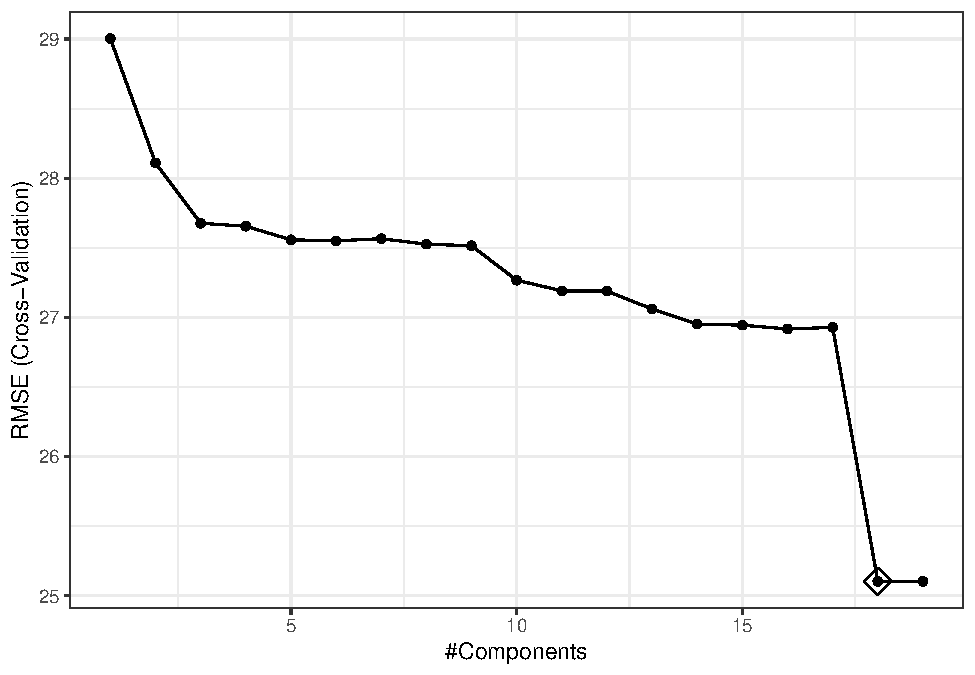
\includegraphics{DSII_final_js5095_files/figure-latex/unnamed-chunk-7-1.pdf}

\begin{Shaded}
\begin{Highlighting}[]
\FunctionTok{ggsave}\NormalTok{(}\StringTok{"pcr.tiff"}\NormalTok{, }\AttributeTok{dpi=}\StringTok{"print"}\NormalTok{)}
\end{Highlighting}
\end{Shaded}

\begin{verbatim}
## Saving 6.5 x 4.5 in image
\end{verbatim}

\hypertarget{pls}{%
\subsection{PLS}\label{pls}}

\begin{Shaded}
\begin{Highlighting}[]
\FunctionTok{set.seed}\NormalTok{(}\DecValTok{1}\NormalTok{)}
\NormalTok{pls.fit }\OtherTok{\textless{}{-}} \FunctionTok{train}\NormalTok{(x.train, y.train,}
                 \AttributeTok{method =} \StringTok{"pls"}\NormalTok{,}
                 \AttributeTok{tuneGrid =} \FunctionTok{data.frame}\NormalTok{(}\AttributeTok{ncomp =} \DecValTok{1}\SpecialCharTok{:}\DecValTok{19}\NormalTok{),}
                 \AttributeTok{trControl =}\NormalTok{ ctrl1,}
                 \AttributeTok{preProcess =} \FunctionTok{c}\NormalTok{(}\StringTok{"center"}\NormalTok{, }\StringTok{"scale"}\NormalTok{))}

\FunctionTok{ggplot}\NormalTok{(pls.fit, }\AttributeTok{highlight =} \ConstantTok{TRUE}\NormalTok{)}
\end{Highlighting}
\end{Shaded}

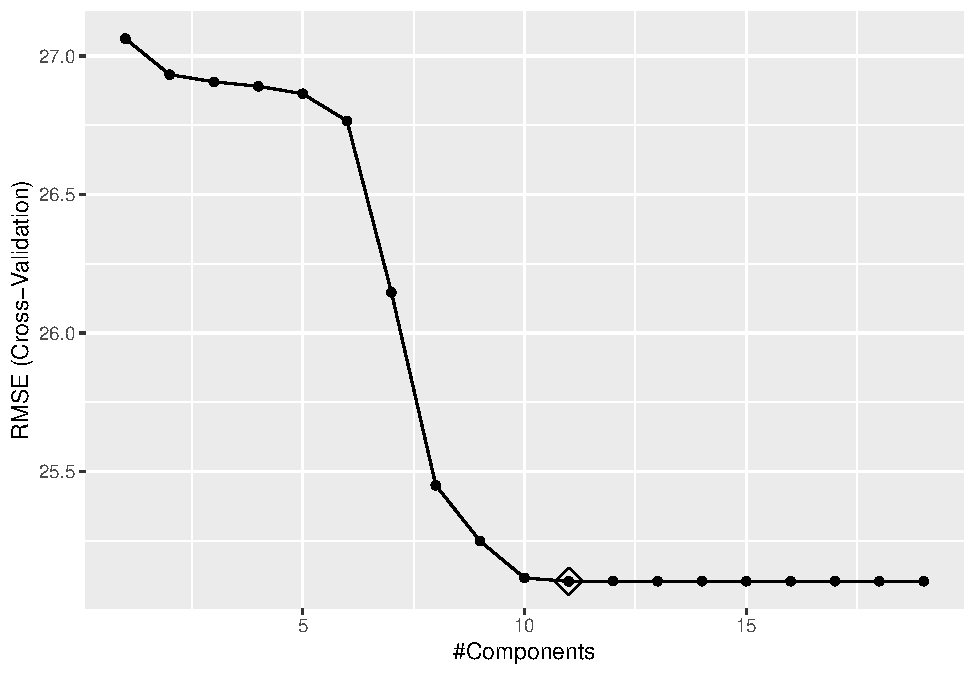
\includegraphics{DSII_final_js5095_files/figure-latex/unnamed-chunk-8-1.pdf}

\begin{Shaded}
\begin{Highlighting}[]
\FunctionTok{ggsave}\NormalTok{(}\StringTok{"pls.tiff"}\NormalTok{, }\AttributeTok{dpi=}\StringTok{"print"}\NormalTok{)}
\end{Highlighting}
\end{Shaded}

\begin{verbatim}
## Saving 6.5 x 4.5 in image
\end{verbatim}

\hypertarget{gam-model}{%
\subsection{GAM model}\label{gam-model}}

\begin{Shaded}
\begin{Highlighting}[]
\FunctionTok{set.seed}\NormalTok{(}\DecValTok{1}\NormalTok{)}
\NormalTok{gam.fit }\OtherTok{\textless{}{-}} \FunctionTok{train}\NormalTok{(x.train, y.train,}
                 \AttributeTok{method =} \StringTok{"gam"}\NormalTok{,}
                 \AttributeTok{tuneGrid =} \FunctionTok{data.frame}\NormalTok{(}\AttributeTok{method =} \StringTok{"GCV.Cp"}\NormalTok{, }\AttributeTok{select =} \FunctionTok{c}\NormalTok{(}\ConstantTok{TRUE}\NormalTok{,}\ConstantTok{FALSE}\NormalTok{)),}
                 \AttributeTok{trControl =}\NormalTok{ ctrl1)}
\end{Highlighting}
\end{Shaded}

\begin{verbatim}
## 载入需要的程辑包:mgcv
\end{verbatim}

\begin{verbatim}
## 载入需要的程辑包:nlme
\end{verbatim}

\begin{verbatim}
## 
## 载入程辑包:'nlme'
\end{verbatim}

\begin{verbatim}
## The following object is masked from 'package:dplyr':
## 
##     collapse
\end{verbatim}

\begin{verbatim}
## This is mgcv 1.8-42. For overview type 'help("mgcv-package")'.
\end{verbatim}

\begin{Shaded}
\begin{Highlighting}[]
\FunctionTok{summary}\NormalTok{(gam.fit)}
\end{Highlighting}
\end{Shaded}

\begin{verbatim}
## 
## Family: gaussian 
## Link function: identity 
## 
## Formula:
## .outcome ~ gender1 + race2 + race3 + race4 + smoking1 + smoking2 + 
##     hypertension1 + diabetes1 + vaccine1 + severity1 + studyB + 
##     studyC + s(age) + s(SBP) + s(LDL) + s(bmi) + s(height) + 
##     s(weight)
## 
## Parametric coefficients:
##               Estimate Std. Error t value Pr(>|t|)    
## (Intercept)    43.2570     1.2848  33.668  < 2e-16 ***
## gender1        -4.7965     0.8214  -5.839 5.84e-09 ***
## race2           0.6993     1.8250   0.383    0.702    
## race3          -1.0536     1.0464  -1.007    0.314    
## race4          -2.0949     1.3842  -1.513    0.130    
## smoking1        4.9659     0.9242   5.373 8.37e-08 ***
## smoking2        7.8849     1.3829   5.702 1.31e-08 ***
## hypertension1   3.4663     0.8248   4.203 2.72e-05 ***
## diabetes1      -0.9107     1.1309  -0.805    0.421    
## vaccine1       -8.0399     0.8415  -9.555  < 2e-16 ***
## severity1       9.4416     1.3296   7.101 1.56e-12 ***
## studyB          4.8228     1.0562   4.566 5.17e-06 ***
## studyC         -0.9022     1.2719  -0.709    0.478    
## ---
## Signif. codes:  0 '***' 0.001 '**' 0.01 '*' 0.05 '.' 0.1 ' ' 1
## 
## Approximate significance of smooth terms:
##                 edf Ref.df       F p-value    
## s(age)    5.732e-09      9   0.000   0.960    
## s(SBP)    7.785e-09      9   0.000   0.757    
## s(LDL)    2.455e-01      9   0.036   0.253    
## s(bmi)    8.737e+00      9 222.822  <2e-16 ***
## s(height) 2.090e-08      9   0.000   0.408    
## s(weight) 1.895e-08      9   0.000   0.446    
## ---
## Signif. codes:  0 '***' 0.001 '**' 0.01 '*' 0.05 '.' 0.1 ' ' 1
## 
## R-sq.(adj) =  0.444   Deviance explained = 44.8%
## GCV = 484.97  Scale est. = 481.27    n = 2882
\end{verbatim}

\begin{Shaded}
\begin{Highlighting}[]
\NormalTok{gam.fit}\SpecialCharTok{$}\NormalTok{bestTune}
\end{Highlighting}
\end{Shaded}

\begin{verbatim}
##   select method
## 2   TRUE GCV.Cp
\end{verbatim}

\begin{Shaded}
\begin{Highlighting}[]
\NormalTok{gam.fit}\SpecialCharTok{$}\NormalTok{finalModel}
\end{Highlighting}
\end{Shaded}

\begin{verbatim}
## 
## Family: gaussian 
## Link function: identity 
## 
## Formula:
## .outcome ~ gender1 + race2 + race3 + race4 + smoking1 + smoking2 + 
##     hypertension1 + diabetes1 + vaccine1 + severity1 + studyB + 
##     studyC + s(age) + s(SBP) + s(LDL) + s(bmi) + s(height) + 
##     s(weight)
## 
## Estimated degrees of freedom:
## 0.000 0.000 0.245 8.737 0.000 0.000  total = 21.98 
## 
## GCV score: 484.9695
\end{verbatim}

\begin{Shaded}
\begin{Highlighting}[]
\FunctionTok{par}\NormalTok{(}\AttributeTok{mfrow =} \FunctionTok{c}\NormalTok{(}\DecValTok{2}\NormalTok{, }\DecValTok{3}\NormalTok{))}

\FunctionTok{plot}\NormalTok{(gam.fit}\SpecialCharTok{$}\NormalTok{finalModel)}
\end{Highlighting}
\end{Shaded}

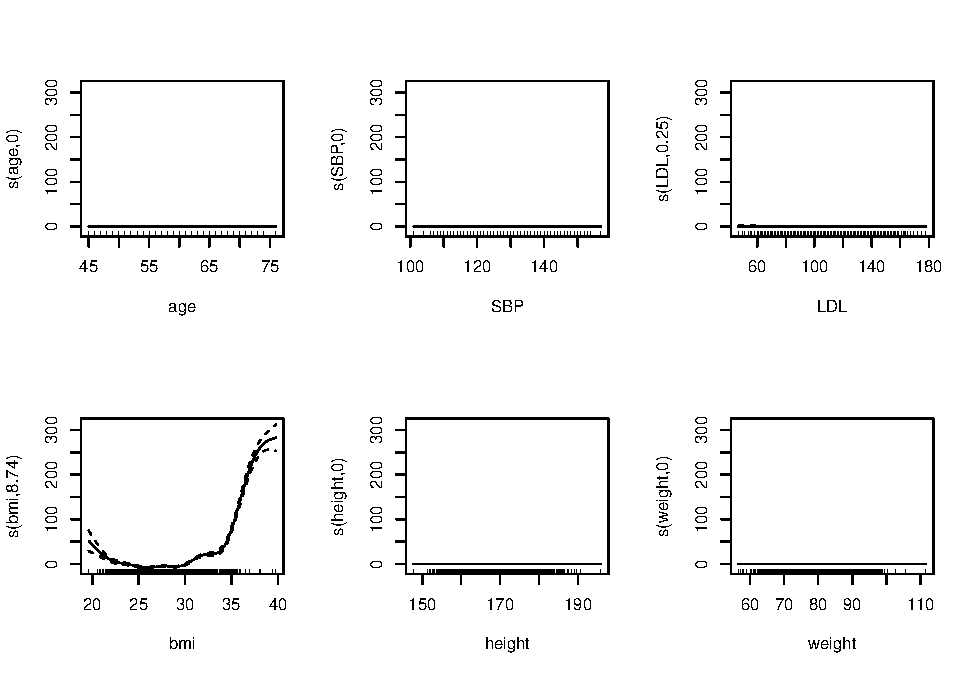
\includegraphics{DSII_final_js5095_files/figure-latex/unnamed-chunk-9-1.pdf}

\hypertarget{mars-model}{%
\subsection{MARS model}\label{mars-model}}

\begin{Shaded}
\begin{Highlighting}[]
\NormalTok{mars\_grid }\OtherTok{\textless{}{-}} \FunctionTok{expand.grid}\NormalTok{(}\AttributeTok{degree =} \DecValTok{1}\SpecialCharTok{:}\DecValTok{3}\NormalTok{, }
                         \AttributeTok{nprune =} \DecValTok{2}\SpecialCharTok{:}\DecValTok{20}\NormalTok{)}

\FunctionTok{set.seed}\NormalTok{(}\DecValTok{1}\NormalTok{)}
\NormalTok{mars.fit }\OtherTok{\textless{}{-}} \FunctionTok{train}\NormalTok{(x.train, y.train,}
                  \AttributeTok{method =} \StringTok{"earth"}\NormalTok{,}
                  \AttributeTok{tuneGrid =}\NormalTok{ mars\_grid,}
                  \AttributeTok{trControl =}\NormalTok{ ctrl1)}
\end{Highlighting}
\end{Shaded}

\begin{verbatim}
## 载入需要的程辑包:earth
\end{verbatim}

\begin{Shaded}
\begin{Highlighting}[]
\FunctionTok{ggplot}\NormalTok{(mars.fit)}
\end{Highlighting}
\end{Shaded}

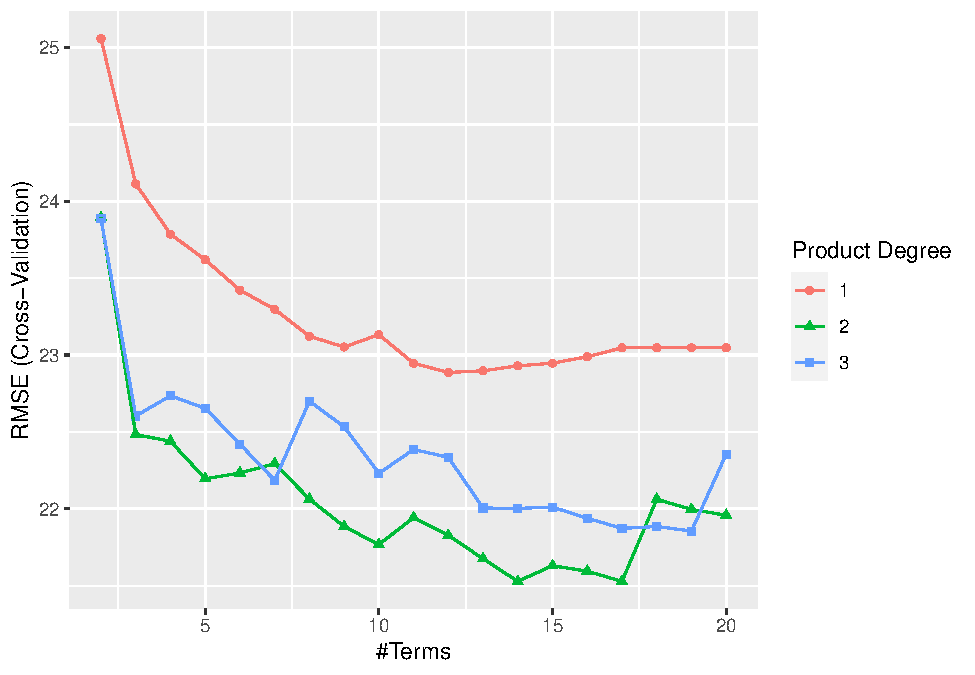
\includegraphics{DSII_final_js5095_files/figure-latex/unnamed-chunk-10-1.pdf}

\begin{Shaded}
\begin{Highlighting}[]
\NormalTok{mars.fit}\SpecialCharTok{$}\NormalTok{bestTune}
\end{Highlighting}
\end{Shaded}

\begin{verbatim}
##    nprune degree
## 35     17      2
\end{verbatim}

\begin{Shaded}
\begin{Highlighting}[]
\FunctionTok{coef}\NormalTok{(mars.fit}\SpecialCharTok{$}\NormalTok{finalModel) }
\end{Highlighting}
\end{Shaded}

\begin{verbatim}
##              (Intercept)              h(33.3-bmi)     h(bmi-33.3) * studyB 
##              -26.8275772                7.5229372               35.5992024 
##                 vaccine1     h(bmi-28.5) * studyB      race4 * h(bmi-33.3) 
##               -7.5760327                6.7123484              -60.2055112 
##  h(bmi-28.5) * severity1   smoking1 * h(bmi-33.3)                  gender1 
##                6.4214446                5.5093431               -4.9104162 
##              h(bmi-23.9) h(bmi-28.5) * h(SBP-138) h(bmi-28.5) * h(SBP-128) 
##                6.9086839               -1.3269459                0.5530760 
##                 smoking1   smoking2 * h(bmi-33.3) h(bmi-33.3) * h(LDL-115) 
##                4.7734050              -54.9024634                0.8394659 
## h(bmi-33.3) * h(115-LDL)   smoking2 * h(bmi-28.5) 
##                0.5197540                8.2746042
\end{verbatim}

\begin{Shaded}
\begin{Highlighting}[]
\FunctionTok{summary}\NormalTok{(mars.fit)}
\end{Highlighting}
\end{Shaded}

\begin{verbatim}
## Call: earth(x=matrix[2882,18], y=c(56,44,53,51,3...), keepxy=TRUE, degree=2,
##             nprune=17)
## 
##                          coefficients
## (Intercept)                -26.827577
## gender1                     -4.910416
## smoking1                     4.773405
## vaccine1                    -7.576033
## h(bmi-23.9)                  6.908684
## h(33.3-bmi)                  7.522937
## race4 * h(bmi-33.3)        -60.205511
## smoking1 * h(bmi-33.3)       5.509343
## smoking2 * h(bmi-33.3)     -54.902463
## smoking2 * h(bmi-28.5)       8.274604
## h(bmi-28.5) * severity1      6.421445
## h(bmi-28.5) * studyB         6.712348
## h(bmi-33.3) * studyB        35.599202
## h(bmi-28.5) * h(SBP-138)    -1.326946
## h(bmi-28.5) * h(SBP-128)     0.553076
## h(bmi-33.3) * h(LDL-115)     0.839466
## h(bmi-33.3) * h(115-LDL)     0.519754
## 
## Selected 17 of 22 terms, and 10 of 18 predictors (nprune=17)
## Termination condition: Reached nk 37
## Importance: bmi, studyB, vaccine1, severity1, race4, SBP, gender1, ...
## Number of terms at each degree of interaction: 1 5 11
## GCV 397.1968    RSS 1112383    GRSq 0.5411432    RSq 0.5537964
\end{verbatim}

\begin{Shaded}
\begin{Highlighting}[]
\FunctionTok{png}\NormalTok{(}\AttributeTok{file=}\StringTok{"mars.png"}\NormalTok{, }\AttributeTok{height=}\DecValTok{1800}\NormalTok{, }\AttributeTok{width=}\DecValTok{1800}\NormalTok{, }\AttributeTok{units =} \StringTok{"px"}\NormalTok{, }\AttributeTok{res=}\DecValTok{200}\NormalTok{)}
\NormalTok{p1 }\OtherTok{\textless{}{-}}\NormalTok{ pdp}\SpecialCharTok{::}\FunctionTok{partial}\NormalTok{(mars.fit, }\AttributeTok{pred.var =} \FunctionTok{c}\NormalTok{(}\StringTok{"bmi"}\NormalTok{), }\AttributeTok{grid.resolution =} \DecValTok{10}\NormalTok{) }\SpecialCharTok{\%\textgreater{}\%} \FunctionTok{autoplot}\NormalTok{()}
\NormalTok{p2 }\OtherTok{\textless{}{-}}\NormalTok{ pdp}\SpecialCharTok{::}\FunctionTok{partial}\NormalTok{(mars.fit, }\AttributeTok{pred.var =} \FunctionTok{c}\NormalTok{(}\StringTok{"height"}\NormalTok{), }\AttributeTok{grid.resolution =} \DecValTok{10}\NormalTok{) }\SpecialCharTok{\%\textgreater{}\%} \FunctionTok{autoplot}\NormalTok{()}
\NormalTok{p3 }\OtherTok{\textless{}{-}}\NormalTok{ pdp}\SpecialCharTok{::}\FunctionTok{partial}\NormalTok{(mars.fit, }\AttributeTok{pred.var =} \FunctionTok{c}\NormalTok{(}\StringTok{"weight"}\NormalTok{), }\AttributeTok{grid.resolution =} \DecValTok{10}\NormalTok{) }\SpecialCharTok{\%\textgreater{}\%} \FunctionTok{autoplot}\NormalTok{()}
\NormalTok{p4 }\OtherTok{\textless{}{-}}\NormalTok{ pdp}\SpecialCharTok{::}\FunctionTok{partial}\NormalTok{(mars.fit, }\AttributeTok{pred.var =} \FunctionTok{c}\NormalTok{(}\StringTok{"bmi"}\NormalTok{, }\StringTok{"height"}\NormalTok{), }
                   \AttributeTok{grid.resolution =} \DecValTok{10}\NormalTok{) }\SpecialCharTok{\%\textgreater{}\%}
\NormalTok{      pdp}\SpecialCharTok{::}\FunctionTok{plotPartial}\NormalTok{(}\AttributeTok{levelplot =} \ConstantTok{FALSE}\NormalTok{, }\AttributeTok{zlab =} \StringTok{"yhat"}\NormalTok{, }\AttributeTok{drape =} \ConstantTok{TRUE}\NormalTok{, }
                       \AttributeTok{screen =} \FunctionTok{list}\NormalTok{(}\AttributeTok{z =} \DecValTok{20}\NormalTok{, }\AttributeTok{x =} \SpecialCharTok{{-}}\DecValTok{60}\NormalTok{))}

\FunctionTok{grid.arrange}\NormalTok{(p1, p2, p3, p4, }\AttributeTok{ncol =} \DecValTok{2}\NormalTok{, }\AttributeTok{nrow =} \DecValTok{2}\NormalTok{)}
\FunctionTok{dev.off}\NormalTok{()}
\end{Highlighting}
\end{Shaded}

\begin{verbatim}
## pdf 
##   2
\end{verbatim}

\hypertarget{regression-tree}{%
\subsection{Regression Tree}\label{regression-tree}}

\begin{Shaded}
\begin{Highlighting}[]
\FunctionTok{set.seed}\NormalTok{(}\DecValTok{1}\NormalTok{)}
\NormalTok{rpart.fit }\OtherTok{\textless{}{-}} \FunctionTok{train}\NormalTok{(}\AttributeTok{x=}\NormalTok{x.train,}
                   \AttributeTok{y =}\NormalTok{ y.train,}
                   \AttributeTok{method =} \StringTok{"rpart"}\NormalTok{,}
                    \AttributeTok{tuneGrid =} \FunctionTok{data.frame}\NormalTok{(}\AttributeTok{cp =} \FunctionTok{exp}\NormalTok{(}\FunctionTok{seq}\NormalTok{(}\SpecialCharTok{{-}}\DecValTok{6}\NormalTok{,}\SpecialCharTok{{-}}\DecValTok{2}\NormalTok{, }\AttributeTok{length =} \DecValTok{50}\NormalTok{))),}
                    \AttributeTok{trControl =}\NormalTok{ ctrl1)}
\end{Highlighting}
\end{Shaded}

\begin{verbatim}
## Warning in nominalTrainWorkflow(x = x, y = y, wts = weights, info = trainInfo,
## : There were missing values in resampled performance measures.
\end{verbatim}

\begin{Shaded}
\begin{Highlighting}[]
\FunctionTok{ggplot}\NormalTok{(rpart.fit, }\AttributeTok{highlight =} \ConstantTok{TRUE}\NormalTok{)}
\end{Highlighting}
\end{Shaded}

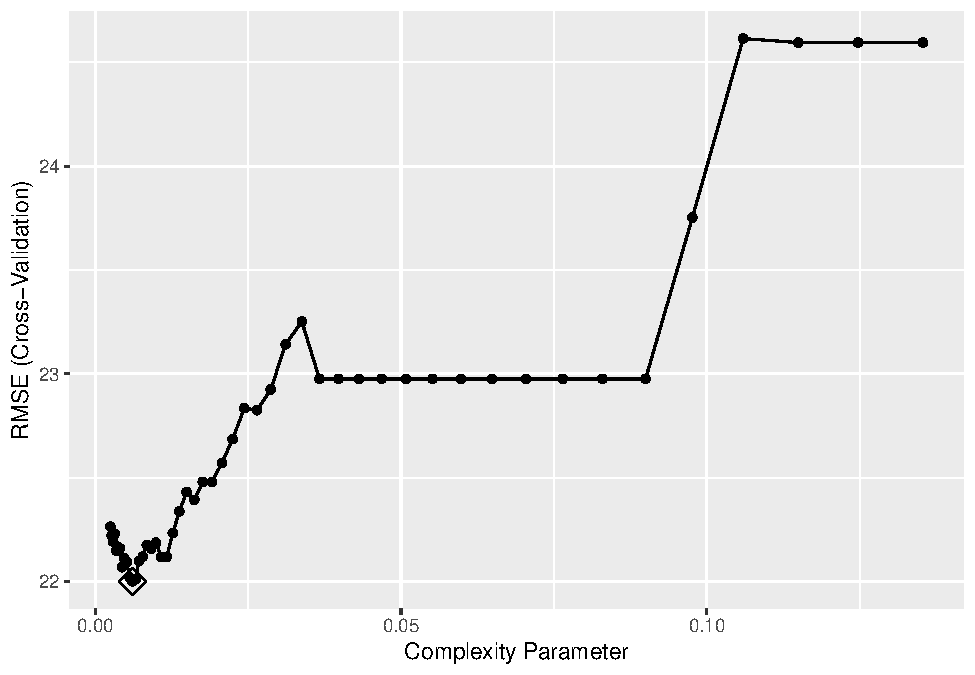
\includegraphics{DSII_final_js5095_files/figure-latex/unnamed-chunk-11-1.pdf}

\begin{Shaded}
\begin{Highlighting}[]
\FunctionTok{rpart.plot}\NormalTok{(rpart.fit}\SpecialCharTok{$}\NormalTok{finalModel)}
\end{Highlighting}
\end{Shaded}

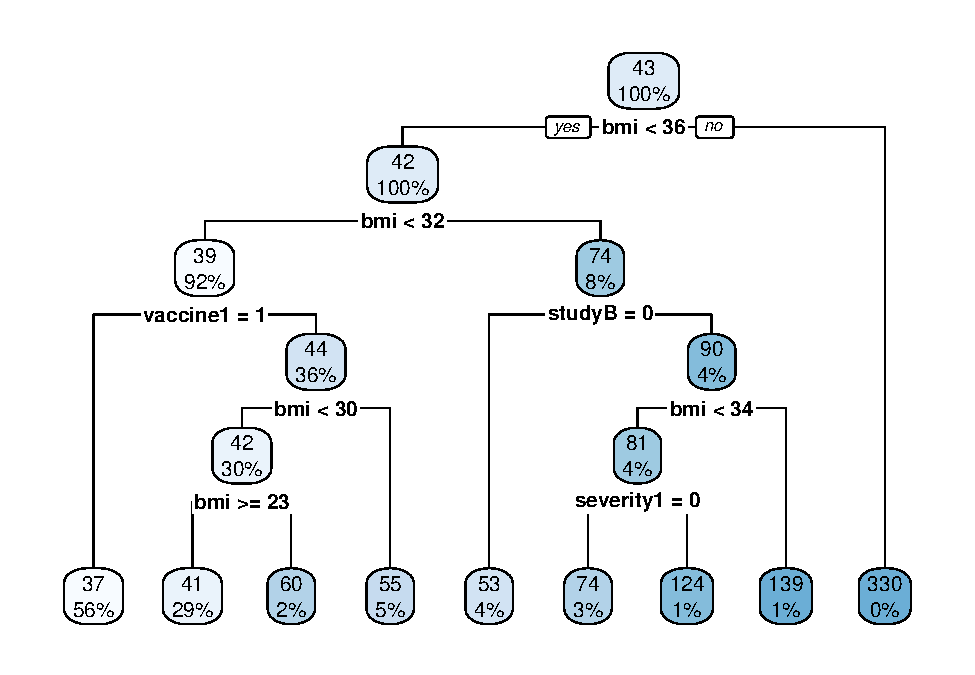
\includegraphics{DSII_final_js5095_files/figure-latex/unnamed-chunk-11-2.pdf}

\hypertarget{random-forest}{%
\subsection{random forest}\label{random-forest}}

\begin{Shaded}
\begin{Highlighting}[]
\CommentTok{\# Try more if possible}
\NormalTok{rf.grid }\OtherTok{\textless{}{-}} \FunctionTok{expand.grid}\NormalTok{(}\AttributeTok{mtry =} \DecValTok{1}\SpecialCharTok{:}\DecValTok{14}\NormalTok{,}
\AttributeTok{splitrule =} \StringTok{"variance"}\NormalTok{,}
\AttributeTok{min.node.size =} \DecValTok{1}\SpecialCharTok{:}\DecValTok{6}\NormalTok{)}
\FunctionTok{set.seed}\NormalTok{(}\DecValTok{1}\NormalTok{)}
\NormalTok{rf.fit }\OtherTok{\textless{}{-}} \FunctionTok{train}\NormalTok{(x.train,}
\NormalTok{                y.train,}
\AttributeTok{method =} \StringTok{"ranger"}\NormalTok{,}
\AttributeTok{tuneGrid =}\NormalTok{ rf.grid,}
\AttributeTok{trControl =}\NormalTok{ ctrl1)}
\end{Highlighting}
\end{Shaded}

\begin{Shaded}
\begin{Highlighting}[]
\FunctionTok{ggplot}\NormalTok{(rf.fit, }\AttributeTok{highlight =} \ConstantTok{TRUE}\NormalTok{)}
\end{Highlighting}
\end{Shaded}

\includegraphics{DSII_final_js5095_files/figure-latex/unnamed-chunk-13-1.pdf}

\begin{Shaded}
\begin{Highlighting}[]
\NormalTok{rf.pred }\OtherTok{\textless{}{-}} \FunctionTok{predict}\NormalTok{(rf.fit, }\AttributeTok{newdata =}\NormalTok{ x.test)}
\FunctionTok{mean}\NormalTok{((y.test}\SpecialCharTok{{-}}\NormalTok{rf.pred)}\SpecialCharTok{\^{}}\DecValTok{2}\NormalTok{)}
\end{Highlighting}
\end{Shaded}

\begin{verbatim}
## [1] 512.5156
\end{verbatim}

\begin{Shaded}
\begin{Highlighting}[]
\NormalTok{gbm.grid }\OtherTok{\textless{}{-}} \FunctionTok{expand.grid}\NormalTok{(}\AttributeTok{n.trees =} \FunctionTok{c}\NormalTok{(}\DecValTok{2000}\NormalTok{,}\DecValTok{4000}\NormalTok{,}\DecValTok{6000}\NormalTok{,}\DecValTok{8000}\NormalTok{,}\DecValTok{10000}\NormalTok{),}
\AttributeTok{interaction.depth =} \DecValTok{1}\SpecialCharTok{:}\DecValTok{3}\NormalTok{,}
\AttributeTok{shrinkage =} \FunctionTok{c}\NormalTok{(}\FloatTok{0.005}\NormalTok{,}\FloatTok{0.01}\NormalTok{),}
\AttributeTok{n.minobsinnode =} \FunctionTok{c}\NormalTok{(}\DecValTok{1}\NormalTok{))}
\FunctionTok{set.seed}\NormalTok{(}\DecValTok{1}\NormalTok{)}
\NormalTok{gbm.fit }\OtherTok{\textless{}{-}} \FunctionTok{train}\NormalTok{(x.train,y.train,}
                 \AttributeTok{method =} \StringTok{"gbm"}\NormalTok{,}
                 \AttributeTok{tuneGrid =}\NormalTok{ gbm.grid,}
                 \AttributeTok{trControl =}\NormalTok{ ctrl1,}
                 \AttributeTok{verbose =} \ConstantTok{FALSE}\NormalTok{)}
\end{Highlighting}
\end{Shaded}

\begin{Shaded}
\begin{Highlighting}[]
\FunctionTok{ggplot}\NormalTok{(gbm.fit, }\AttributeTok{highlight =} \ConstantTok{TRUE}\NormalTok{)}
\end{Highlighting}
\end{Shaded}

\includegraphics{DSII_final_js5095_files/figure-latex/unnamed-chunk-16-1.pdf}

\begin{Shaded}
\begin{Highlighting}[]
\NormalTok{gbm.pred }\OtherTok{\textless{}{-}} \FunctionTok{predict}\NormalTok{(gbm.fit, }\AttributeTok{newdata =}\NormalTok{ x.test)}
\FunctionTok{mean}\NormalTok{((y.test}\SpecialCharTok{{-}}\NormalTok{gbm.pred)}\SpecialCharTok{\^{}}\DecValTok{2}\NormalTok{)}
\end{Highlighting}
\end{Shaded}

\begin{verbatim}
## [1] 487.4652
\end{verbatim}

\begin{Shaded}
\begin{Highlighting}[]
\FunctionTok{set.seed}\NormalTok{(}\DecValTok{1}\NormalTok{)}
\NormalTok{rf2.final.per }\OtherTok{\textless{}{-}} \FunctionTok{ranger}\NormalTok{(recovery\_time}\SpecialCharTok{\textasciitilde{}}\NormalTok{., dat1[trainRows,],}
                        \AttributeTok{mtry =}\NormalTok{ rf.fit}\SpecialCharTok{$}\NormalTok{bestTune[[}\DecValTok{1}\NormalTok{]],}
                        \AttributeTok{splitrule =} \StringTok{"variance"}\NormalTok{,}
                        \AttributeTok{min.node.size =}\NormalTok{ rf.fit}\SpecialCharTok{$}\NormalTok{bestTune[[}\DecValTok{3}\NormalTok{]],}
                        \AttributeTok{importance =} \StringTok{"permutation"}\NormalTok{,}
                         \AttributeTok{scale.permutation.importance =} \ConstantTok{TRUE}\NormalTok{)}

\FunctionTok{barplot}\NormalTok{(}\FunctionTok{sort}\NormalTok{(ranger}\SpecialCharTok{::}\FunctionTok{importance}\NormalTok{(rf2.final.per), }\AttributeTok{decreasing =} \ConstantTok{FALSE}\NormalTok{),}
\AttributeTok{las =} \DecValTok{2}\NormalTok{, }\AttributeTok{horiz =} \ConstantTok{TRUE}\NormalTok{, }\AttributeTok{cex.names =} \FloatTok{0.7}\NormalTok{,}
\AttributeTok{col =} \FunctionTok{colorRampPalette}\NormalTok{(}\AttributeTok{colors =} \FunctionTok{c}\NormalTok{(}\StringTok{"cyan"}\NormalTok{,}\StringTok{"blue"}\NormalTok{))(}\DecValTok{19}\NormalTok{))}
\end{Highlighting}
\end{Shaded}

\includegraphics{DSII_final_js5095_files/figure-latex/unnamed-chunk-17-1.pdf}

\begin{Shaded}
\begin{Highlighting}[]
\FunctionTok{summary}\NormalTok{(gbm.fit}\SpecialCharTok{$}\NormalTok{finalModel, }\AttributeTok{las =} \DecValTok{2}\NormalTok{, }\AttributeTok{cBars =} \DecValTok{19}\NormalTok{, }\AttributeTok{cex.names =} \FloatTok{0.6}\NormalTok{)}
\end{Highlighting}
\end{Shaded}

\includegraphics{DSII_final_js5095_files/figure-latex/unnamed-chunk-18-1.pdf}

\begin{verbatim}
##                         var     rel.inf
## bmi                     bmi 67.98507215
## studyB               studyB 11.04019125
## height               height  3.11027713
## vaccine1           vaccine1  2.80598010
## severity1         severity1  2.41754331
## SBP                     SBP  2.19109833
## weight               weight  2.15794966
## LDL                     LDL  1.91344748
## age                     age  1.47161785
## smoking2           smoking2  1.45559538
## gender1             gender1  1.25955715
## smoking1           smoking1  1.09018405
## studyC               studyC  0.34773985
## race4                 race4  0.34765420
## race3                 race3  0.27311430
## race2                 race2  0.05118855
## hypertension1 hypertension1  0.04612109
## diabetes1         diabetes1  0.03566815
\end{verbatim}

\hypertarget{comparing-different-models}{%
\subsection{Comparing different
models}\label{comparing-different-models}}

\begin{Shaded}
\begin{Highlighting}[]
\FunctionTok{set.seed}\NormalTok{(}\DecValTok{1}\NormalTok{)}
\NormalTok{resamp }\OtherTok{=} \FunctionTok{resamples}\NormalTok{(}\FunctionTok{list}\NormalTok{(}\AttributeTok{enet =}\NormalTok{ enet.fit, }\AttributeTok{pls =}\NormalTok{ pls.fit, }\AttributeTok{gam =}\NormalTok{ gam.fit, }\AttributeTok{mars =}\NormalTok{ mars.fit,}\AttributeTok{rf =}\NormalTok{ rf.fit,}\AttributeTok{gbm =}\NormalTok{ gbm.fit, }\AttributeTok{rpart =}\NormalTok{ rpart.fit))}
\FunctionTok{summary}\NormalTok{(resamp)}
\end{Highlighting}
\end{Shaded}

\begin{verbatim}
## 
## Call:
## summary.resamples(object = resamp)
## 
## Models: enet, pls, gam, mars, rf, gbm, rpart 
## Number of resamples: 10 
## 
## MAE 
##           Min.  1st Qu.   Median     Mean  3rd Qu.     Max. NA's
## enet  14.89563 15.41241 16.31429 16.48704 17.18978 18.68102    0
## pls   14.88596 15.73014 16.78619 16.77285 17.65509 18.70689    0
## gam   13.63349 14.66753 15.56539 15.39251 16.01871 16.82288    0
## mars  13.57177 14.17293 14.70892 14.88652 15.85824 16.12610    0
## rf    13.34452 13.71658 14.81148 14.75197 15.67082 16.18638    0
## gbm   12.80459 13.54969 14.46672 14.36228 15.21148 15.78439    0
## rpart 13.57200 14.43384 15.08326 15.06314 15.64389 16.76941    0
## 
## RMSE 
##           Min.  1st Qu.   Median     Mean  3rd Qu.     Max. NA's
## enet  21.66236 23.10295 24.43842 25.55056 27.18938 34.24423    0
## pls   21.69353 23.36433 24.10026 25.10344 26.34144 32.59019    0
## gam   18.59663 20.80165 22.51682 22.46502 24.35001 26.14106    0
## mars  18.32398 19.83786 20.97298 21.52795 23.18857 25.77849    0
## rf    17.91126 19.56908 21.34942 21.33878 23.27605 23.97571    0
## gbm   16.99334 19.28323 21.00432 20.63349 22.20037 23.10783    0
## rpart 18.10205 20.48515 21.60586 22.00056 24.17166 26.08592    0
## 
## Rsquared 
##             Min.   1st Qu.    Median      Mean   3rd Qu.      Max. NA's
## enet  0.08983837 0.1977097 0.2506698 0.2393136 0.2882582 0.3466723    0
## pls   0.11783579 0.2047681 0.2671251 0.2632351 0.3365684 0.3870614    0
## gam   0.14925569 0.3053848 0.4458158 0.4177506 0.5275640 0.6443694    0
## mars  0.14582135 0.3633383 0.4571700 0.4526473 0.5790718 0.6588231    0
## rf    0.14785585 0.3680986 0.4628669 0.4531400 0.5706298 0.6700218    0
## gbm   0.14759097 0.4206024 0.4852933 0.4842539 0.6221652 0.7058248    0
## rpart 0.02935530 0.3516698 0.4622695 0.4285523 0.5761503 0.6673153    0
\end{verbatim}

\begin{Shaded}
\begin{Highlighting}[]
\FunctionTok{parallelplot}\NormalTok{(resamp, }\AttributeTok{metric =} \StringTok{"RMSE"}\NormalTok{)}
\end{Highlighting}
\end{Shaded}

\includegraphics{DSII_final_js5095_files/figure-latex/unnamed-chunk-19-1.pdf}

\begin{Shaded}
\begin{Highlighting}[]
\FunctionTok{png}\NormalTok{(}\AttributeTok{file=}\StringTok{"comparison.png"}\NormalTok{, }\AttributeTok{height=}\DecValTok{1800}\NormalTok{, }\AttributeTok{width=}\DecValTok{1800}\NormalTok{, }\AttributeTok{units =} \StringTok{"px"}\NormalTok{, }\AttributeTok{res=}\DecValTok{200}\NormalTok{)}
\FunctionTok{bwplot}\NormalTok{(resamp, }\AttributeTok{metric =} \StringTok{"RMSE"}\NormalTok{)}
\end{Highlighting}
\end{Shaded}

\hypertarget{section}{%
\subsection{}\label{section}}

\begin{Shaded}
\begin{Highlighting}[]
\FunctionTok{png}\NormalTok{(}\AttributeTok{file=}\StringTok{"VIP.png"}\NormalTok{, }\AttributeTok{height=}\DecValTok{1800}\NormalTok{, }\AttributeTok{width=}\DecValTok{1800}\NormalTok{, }\AttributeTok{units =} \StringTok{"px"}\NormalTok{, }\AttributeTok{res=}\DecValTok{200}\NormalTok{)}
\NormalTok{p1 }\OtherTok{\textless{}{-}} \FunctionTok{vip}\NormalTok{(mars.fit, }\AttributeTok{num\_features =} \DecValTok{40}\NormalTok{, }\AttributeTok{bar =} \ConstantTok{FALSE}\NormalTok{, }\AttributeTok{value =} \StringTok{"gcv"}\NormalTok{) }\SpecialCharTok{+} \FunctionTok{ggtitle}\NormalTok{(}\StringTok{"GCV"}\NormalTok{)}
\NormalTok{p2 }\OtherTok{\textless{}{-}} \FunctionTok{vip}\NormalTok{(mars.fit, }\AttributeTok{num\_features =} \DecValTok{40}\NormalTok{, }\AttributeTok{bar =} \ConstantTok{FALSE}\NormalTok{, }\AttributeTok{value =} \StringTok{"rss"}\NormalTok{) }\SpecialCharTok{+} \FunctionTok{ggtitle}\NormalTok{(}\StringTok{"RSS"}\NormalTok{)}

\NormalTok{gridExtra}\SpecialCharTok{::}\FunctionTok{grid.arrange}\NormalTok{(p1, p2, }\AttributeTok{ncol =} \DecValTok{2}\NormalTok{)}
\FunctionTok{dev.off}\NormalTok{()}
\end{Highlighting}
\end{Shaded}

\begin{verbatim}
## pdf 
##   2
\end{verbatim}

\hypertarget{prediction}{%
\subsection{Prediction}\label{prediction}}

\begin{Shaded}
\begin{Highlighting}[]
\NormalTok{predy2.pls }\OtherTok{=} \FunctionTok{predict}\NormalTok{(lm.fit, }\AttributeTok{newdata =}\NormalTok{ x.test)}
\FunctionTok{mean}\NormalTok{((y.test}\SpecialCharTok{{-}}\NormalTok{predy2.pls)}\SpecialCharTok{\^{}}\DecValTok{2}\NormalTok{)}
\end{Highlighting}
\end{Shaded}

\begin{verbatim}
## [1] 652.6144
\end{verbatim}

\begin{Shaded}
\begin{Highlighting}[]
\NormalTok{predy2.pls }\OtherTok{=} \FunctionTok{predict}\NormalTok{(ridge.fit, }\AttributeTok{newdata =}\NormalTok{ x.test)}
\FunctionTok{mean}\NormalTok{((y.test}\SpecialCharTok{{-}}\NormalTok{predy2.pls)}\SpecialCharTok{\^{}}\DecValTok{2}\NormalTok{)}
\end{Highlighting}
\end{Shaded}

\begin{verbatim}
## [1] 745.3525
\end{verbatim}

\begin{Shaded}
\begin{Highlighting}[]
\NormalTok{predy2.pls }\OtherTok{=} \FunctionTok{predict}\NormalTok{(enet.fit, }\AttributeTok{newdata =}\NormalTok{ x.test)}
\FunctionTok{mean}\NormalTok{((y.test}\SpecialCharTok{{-}}\NormalTok{predy2.pls)}\SpecialCharTok{\^{}}\DecValTok{2}\NormalTok{)}
\end{Highlighting}
\end{Shaded}

\begin{verbatim}
## [1] 677.4994
\end{verbatim}

\begin{Shaded}
\begin{Highlighting}[]
\NormalTok{predy2.pls }\OtherTok{=} \FunctionTok{predict}\NormalTok{(pls.fit, }\AttributeTok{newdata =}\NormalTok{ x.test)}
\FunctionTok{mean}\NormalTok{((y.test}\SpecialCharTok{{-}}\NormalTok{predy2.pls)}\SpecialCharTok{\^{}}\DecValTok{2}\NormalTok{)}
\end{Highlighting}
\end{Shaded}

\begin{verbatim}
## [1] 652.476
\end{verbatim}

\begin{Shaded}
\begin{Highlighting}[]
\NormalTok{predy2.pcr }\OtherTok{=} \FunctionTok{predict}\NormalTok{(pcr.fit, }\AttributeTok{newdata =}\NormalTok{ x.test)}
\FunctionTok{mean}\NormalTok{((y.test}\SpecialCharTok{{-}}\NormalTok{predy2.pcr)}\SpecialCharTok{\^{}}\DecValTok{2}\NormalTok{)}
\end{Highlighting}
\end{Shaded}

\begin{verbatim}
## [1] 652.6144
\end{verbatim}

\begin{Shaded}
\begin{Highlighting}[]
\NormalTok{predy2.mars }\OtherTok{=} \FunctionTok{predict}\NormalTok{(mars.fit, }\AttributeTok{newdata =}\NormalTok{ x.test)}
\FunctionTok{mean}\NormalTok{((y.test}\SpecialCharTok{{-}}\NormalTok{predy2.mars)}\SpecialCharTok{\^{}}\DecValTok{2}\NormalTok{)}
\end{Highlighting}
\end{Shaded}

\begin{verbatim}
## [1] 439.1718
\end{verbatim}

\begin{Shaded}
\begin{Highlighting}[]
\NormalTok{predy2.lasso }\OtherTok{=} \FunctionTok{predict}\NormalTok{(lasso.fit, }\AttributeTok{newdata =}\NormalTok{ x.test)}
\FunctionTok{mean}\NormalTok{((y.test}\SpecialCharTok{{-}}\NormalTok{predy2.lasso)}\SpecialCharTok{\^{}}\DecValTok{2}\NormalTok{)}
\end{Highlighting}
\end{Shaded}

\begin{verbatim}
## [1] 652.7542
\end{verbatim}

\begin{Shaded}
\begin{Highlighting}[]
\NormalTok{predy2.gam }\OtherTok{=} \FunctionTok{predict}\NormalTok{(gam.fit, }\AttributeTok{newdata =}\NormalTok{ x.test)}
\FunctionTok{mean}\NormalTok{((y.test}\SpecialCharTok{{-}}\NormalTok{predy2.gam)}\SpecialCharTok{\^{}}\DecValTok{2}\NormalTok{)}
\end{Highlighting}
\end{Shaded}

\begin{verbatim}
## [1] 486.8146
\end{verbatim}

\end{document}
